\chapter{The Silicon Detector Array}
In order to take advantage of the HELIOS concept, the light ion reaction products transported through the HELIOS solenoid must be detected in a slender array close to the beam axis.  The radial extent of the array should be on the order of 1\,cm.  For rearward hemisphere operation, the array must also be hollow to permit the transmission of the beam to the target foil.  The silicon detectors which  make up the array must be position sensitive along their length with a position resolution on the order of $\delta z = 0.5$--1.0\,mm~FWHM.  In addition, the intrinsic detector energy resolution should be on the order of $\delta E_\mathrm{lab} =25$--50\,keV~FWHM.  This chapter describes characterization and construction of the silicon detector array as they relate to these design requirements.
\section{The Detectors}
\label{detectors}
\subsection{Specifications}
The prototype array utilizes detectors that were manufactured by Canberra Industries.  The detectors were designed for and used in a previous application as a nuclear reaction calorimeter~\cite[pp. 100--104]{Blumenthal_PhD}.  The detectors are position-sensitive passivated implanted planar silicon detectors.  The detectors are 12\,mm $\times$ 56\,mm silicon wafers, $700\pm15$\,$\mu$m thick\footnote{Thickness quoted in private communication from the manufacturer.} with active areas 9\,mm $\times$ 50.5\,mm.  The particle energy which this detector thickness is capable of stopping is shown in Table~\ref{srim} for a number of light ions.

The construction of the detectors follows the standard fabrication method of passivated implanted planar silicon detectors~\cite{Kemmer_1984}.  First the edges of the silicon wafers are passivated by thermal oxidation which, after etching, produces an insulating boundary of SiO. Next the front of each detector (the side shown in Fig.~\ref{pcb}) is implanted with boron ions to form a p$^+$n junction and the back of the detectors is implanted with arsenic to form an n-type junction.  Then after annealing, aluminum contacts, discussed below, are patterned on either side of the detector for electrical connections.  The thin layer of boron provides position sensitivity along the length  of the detector by resistive division.  The dead layer introduced by the ohmic contact on the back of the detector---typically the entrance window---is equivalent to a silicon thickness of $<50$\,nm.  The dead layer on the junction side is $<100$\,nm silicon equivalent.  A typical detector is fully depleted at a reverse-bias voltage of 190\,V producing nominal leakage current of 350\,nA.

\begin{table}
  \begin{center}
    \begin{tabular}{c..}
      \hline
      \multicolumn{1}{c}{\multirow{2}{*}{Nucleon}}  &
    	\multicolumn{2}{c}{Incidence Angle}\\ \cline{2-3}
    	&\multicolumn{1}{c}{$\vartheta=0^\circ$}&\multicolumn{1}{c}{$\vartheta=45^\circ$}\\\hline \hline 
      $p$&9.9&12.1\\
      $d$&13.2&16.2\\
      $t$&15.7&19.2\\
      $^3$He&35.1&42.9\\
      $\alpha$&39.6&48.7\\\hline
    \end{tabular}
    \label{srim}
    \caption[Stopping power calculations for the HELIOS silicon detectors]{Stopping power calculations for the HELIOS silicon detectors.  Approximate light ion energies in MeV with stopping ranges of 700\,$\mu$m for two different incident angles $\vartheta$ are given.  The calculations were carried out using the Monte Carlo simulation program SRIM (Stopping and Range of Ions in Matter), which has reported accuracy of 4.3\%~\cite{Ziegler_2010}.}
  \end{center}
\end{table}

\begin{figure}[t]
\centering
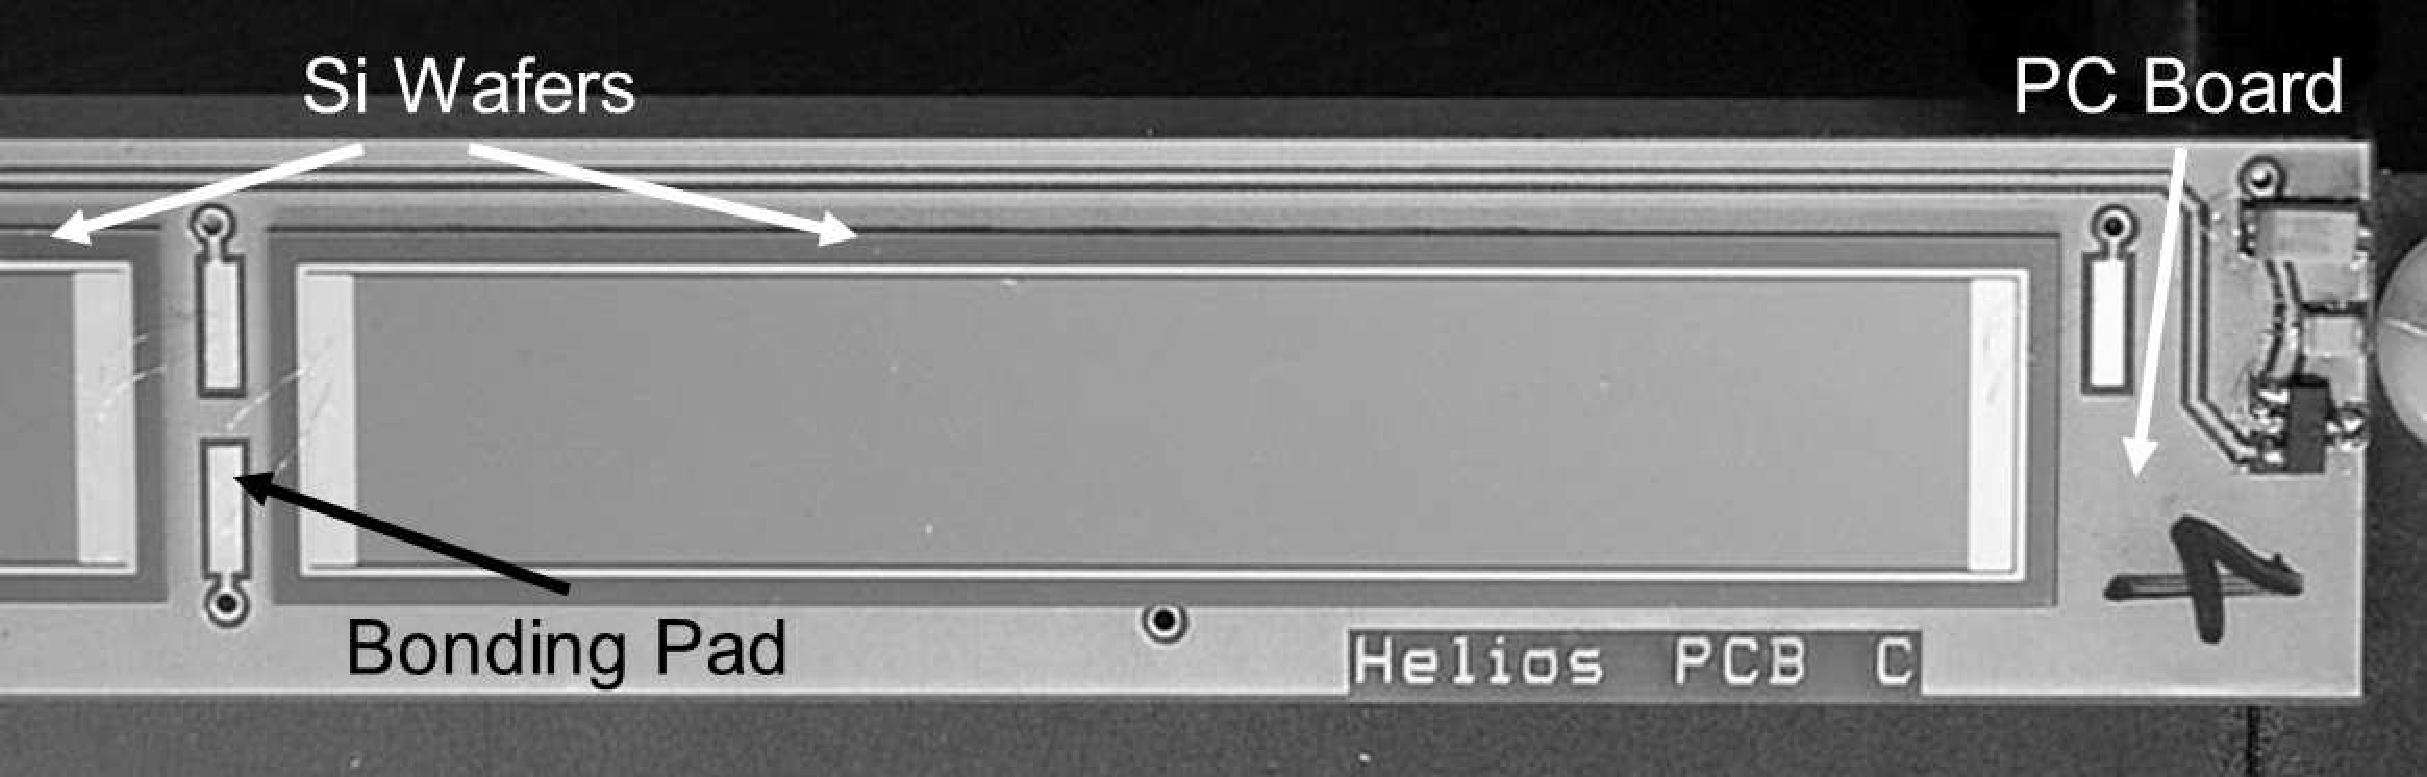
\includegraphics[width=\linewidth]{../NIM_Paper/Figures/BW_Figures/pcb2_bw}
\caption[Detail of a silicon detector mounted on a modular section of the HELIOS silicon detector array]{Detail of a silicon detector mounted on a modular section of the HELIOS silicon detector array.  Dual bonding wires connect each end of the detector to the PC board.  On the detector shown, the guard ring is connected to the left-hand side bonding pad.  The target-end of the PC board (right-hand side in the figure) features a temperature sensor.    Photo by A.~H.\ Wuosmaa, \photodate\formatdate{26}{2}{2008}.  This figure also appears in Ref.~\cite{Lighthall_2010}.}
\label{pcb}
\end{figure}

Each detector has three aluminum signal contacts; one covering the back of the detector and one at each end of the front of the detector.  The implanted resistive layer provides about 17\,k$\Omega$ of resistance between the two front contacts.  One of the contacts is also connected to a guard ring that separates the active area of the detector from the oxide passivated edges of the detector.  This guard ring helps define the electric field along the edges of the detector.  The position signals may be read out from the bonding pads at either end of the detector as shown in Fig.~\ref{pcb}.  In addition, the total energy of the detected ions is measured from the contact at back of the detector.  With the position signals identified as $X_\mathrm{far}$ and $X_\mathrm{near}$, with ``far'' and ``near'' relative to say, the target, the position on the detector is defined as 

\begin{equation}
\begin{split}
X=&\frac{L}{2}\left[1+\frac{(X_\mathrm{far}-X_\mathrm{near})}{E}\right]
%=&\frac{L}{2}\left[1+\frac{(X_\mathrm{far}-X_\mathrm{near})}{(X_\mathrm{far}+X_\mathrm{near})}\right]
\label{detector_X}
\end{split}
\end{equation}

with $X=0$ corresponding to an event at the $X_\mathrm{near}$ end of the detector and $X=L$ corresponding to an event at the $X_\mathrm{far}$ end, where $L=50.5$\,mm, the length of the detector.

However, all three signals need not be measured in order determine the position of a detected ion.  When the detectors were used in the nuclear calorimeter, only two channels were read out for each detector.  The bonding pad connected to the guard ring was grounded and the position was signal was read out only from the contact at the other end of the detector.  The ratio of the position signal to the energy signal was then used to determine the position. % using the relation $X=L[X_\mathrm{single}/E]$.
The position can be determined using any two of the available measured quantities.

\begin{subequations}
\label{detector_redund}
\begin{eqnarray}
%\begin{split}
X=\frac{L}{2}\left[1+\frac{(X_\mathrm{far}-X_\mathrm{near})}{(X_\mathrm{far}+X_\mathrm{near})}\right]\qquad& \textrm{without E}\label{x_noE}\\
X=L\left[\frac{X_\mathrm{far}}{E}\right]\qquad& \textrm{without }X_\mathrm{near}\label{x_noXN}\\
X=L\left[1-\frac{X_\mathrm{near}}{E}\right]\qquad& \textrm{without }X_\mathrm{far}\label{x_noXF}
%\end{split}
\end{eqnarray}
\end{subequations}
Measuring all three quantities leaves the system over-determined and and has a number of advantages.  In the HELIOS configuration, reading out both position signals provides a redundant energy measurement.  And as will be explained in Chapt.~\ref{calib}, reading out all three signals also allows for noise rejection. 

\subsection{Characterization}
\label{charact}
The HELIOS PSD detectors were characterized at Western Michigan University using both an $^{241}$Am radioactive decay source and the Physics Department's model EN 6.0\,MeV tandem Van de Graaff accelerator.  The results of the characterization experiments are reported briefly in Ref.~\cite{Lighthall_2010}; this section expands on that discussion and details additional measurements.  The accelerator tests were carried out over a time period between October, 2006 and March, 2007.  Fig.~\ref{test_mount} shows the testing mount that was used, including the scattering mask that was used to assess the position resolution of the detectors.

\begin{figure}
\centering
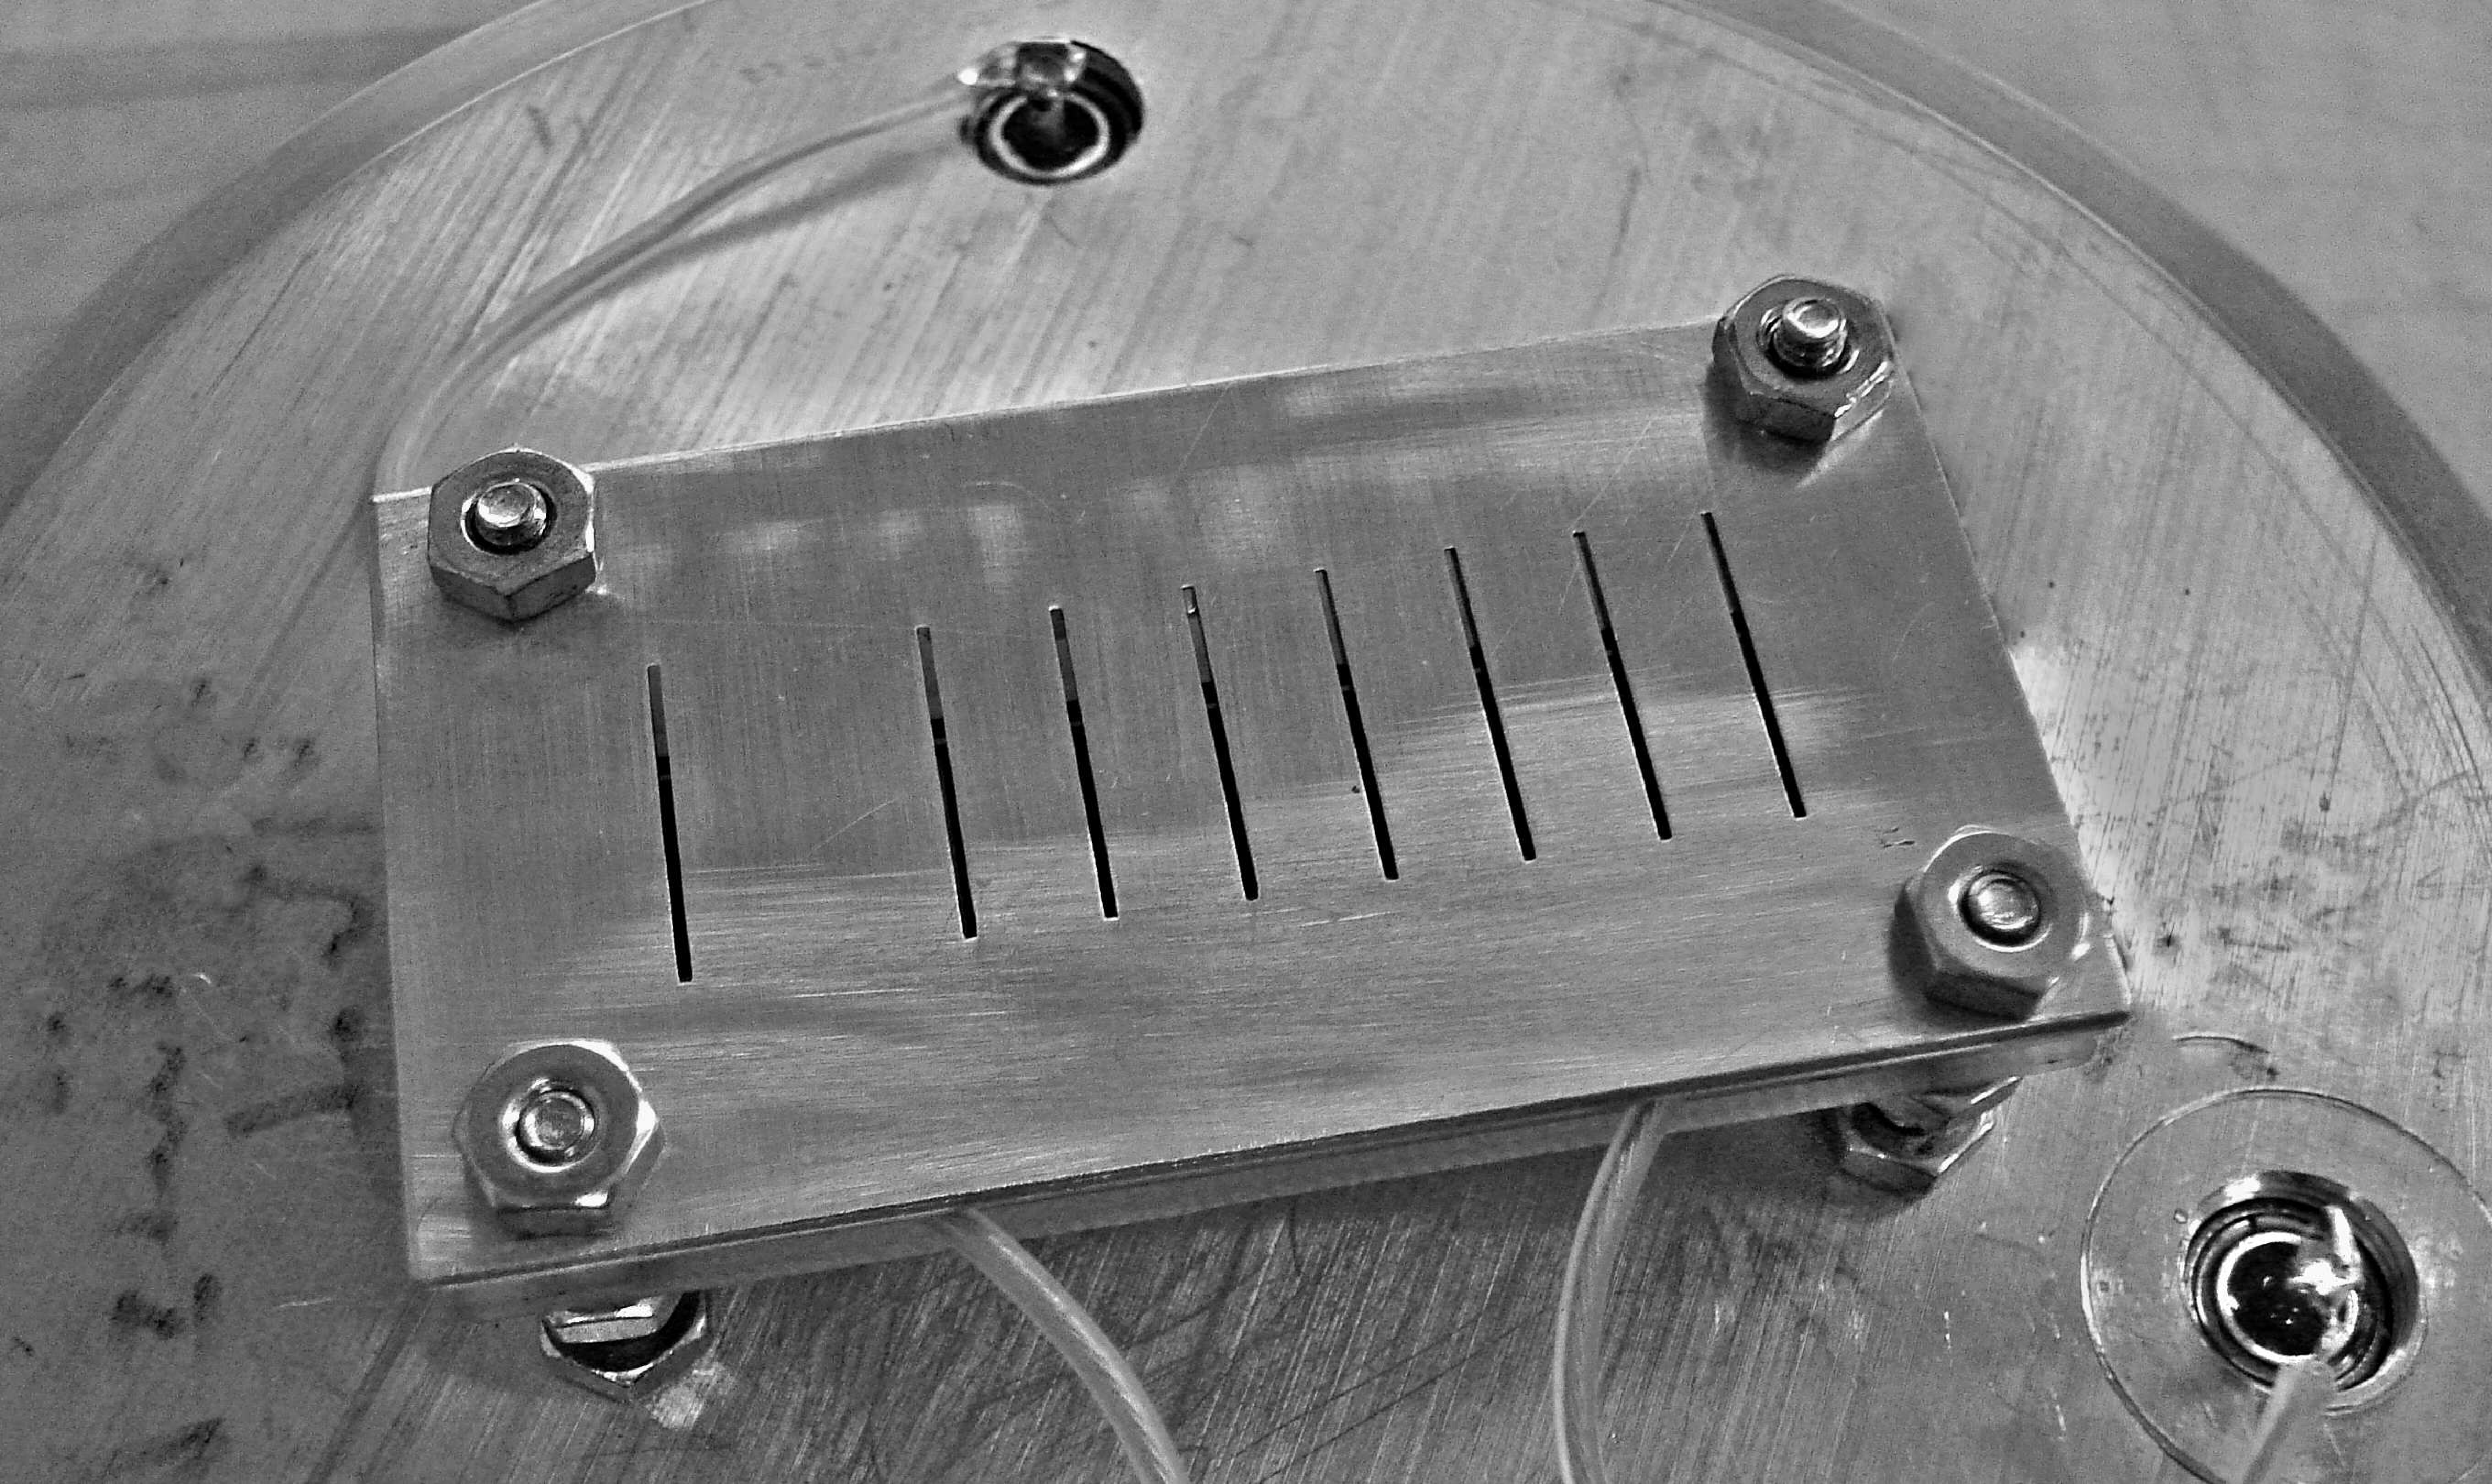
\includegraphics[width=\columnwidth,height=0.4\textheight,keepaspectratio]{DSC00508}%
\caption[Testing mount for the PSD characterization, including the scattering mask]{Testing mount for the PSD characterization, including the scattering mask.  The detector is clamped between two fiberglass frames (hidden) which provide the electrical contacts.  The electric connection between the frames and the detector is made with conductive rubber pads.  The mask measure 30\,mm $\times$ 60\,mm.}%
\label{test_mount}%
\end{figure}

\subsubsection{Position \& Energy}
The position and energy resolutions were measured by elastic scattering of a proton beam at four different energies from a carbon foil into an individual, masked detector.  The detector was positioned at a radius of 105\,mm from the beam axis with a proton scattering angle of $\theta_\mathrm{lab}=60^\circ$ corresponding to normal incidence at the center of the detector.  The experimental setup is shown in Fig.~\ref{scat_setup}.  The results of these runs are shown in Fig.~\ref{psd_test}.  The symmetric U-shaped energy cutoff at low energy is due to an electronic threshold of 112\,keV on all three signals, as indicated by the dashed curve in the figure.

\begin{figure}%
\centering
\hspace*{\stretch{1}}%
\fbox{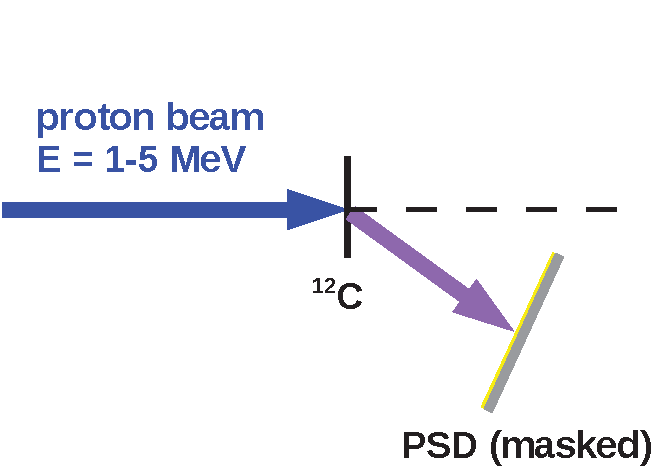
\includegraphics[height=0.2\textheight,keepaspectratio]{dnp08_stm_1}}\hspace*{\stretch{1}}
\fbox{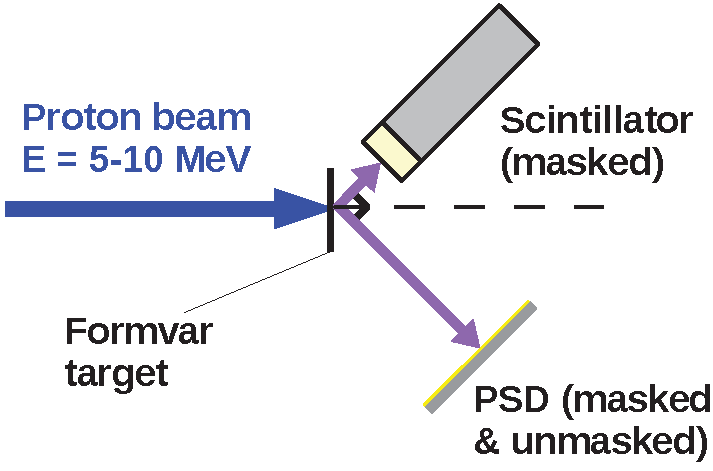
\includegraphics[height=0.2\textheight,keepaspectratio]{dnp08_stm_2}}\hspace*{\stretch{1}}
\caption[Scattering chamber setup for the PSD characterization experiments]{Scattering chamber setup for the PSD characterization experiments.  (left) For the position, energy, and length measurements, a masked detector was placed at $\theta_\mathrm{lab}=60^\circ$ to measure elastic $^{12}$C($p$,$p$) scattering. (right) For the timing measurements a scintillator and a silicon detector were placed 90$^\circ$ apart at $\theta_\mathrm{lab}=\pm45^\circ$ to measure elastic $^1$H($p$,$p$) scattering.  Figure from Ref.~\cite{Marley_2008}.}
\label{scat_setup}%
\end{figure}

\begin{figure*}
\centering
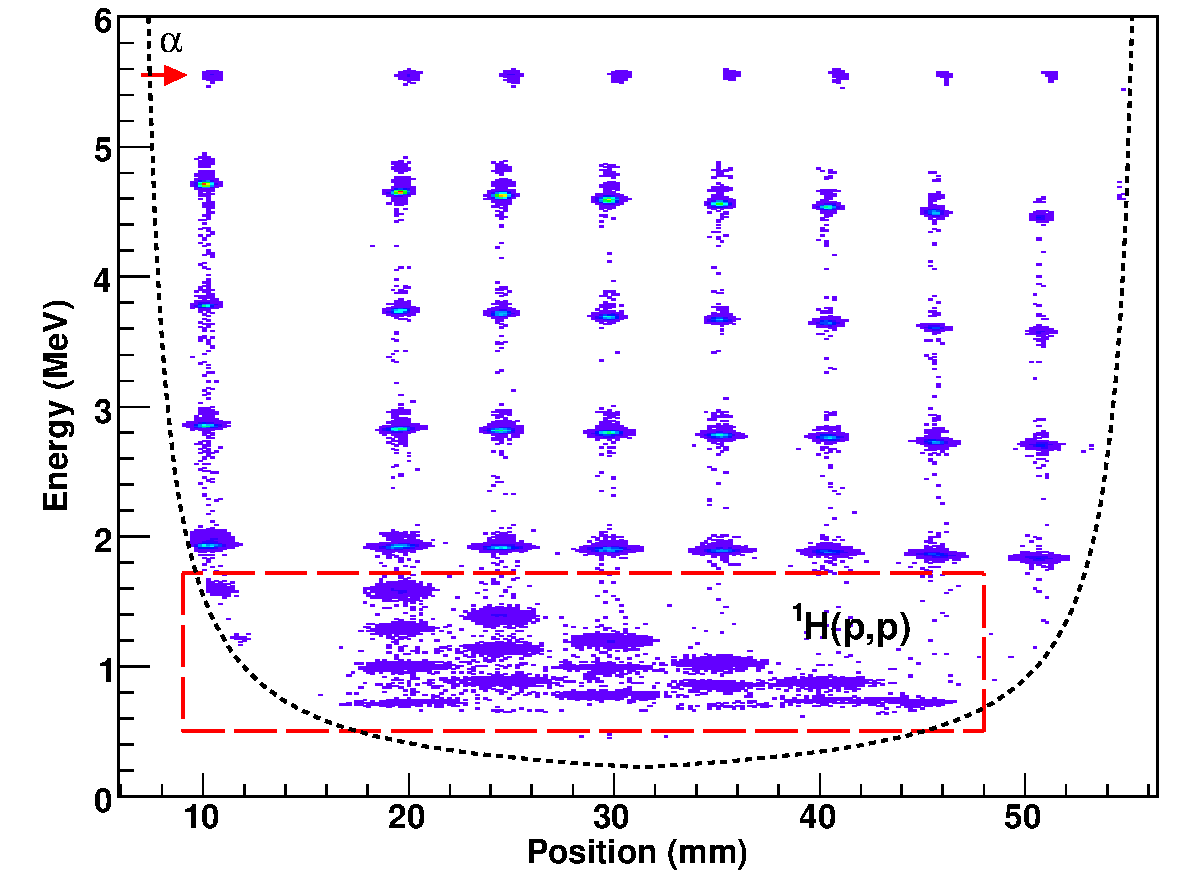
\includegraphics[width=\linewidth]{Figures/out1}
\caption[Characteristic energy versus position spectrum of a HELIOS PSD]{Characteristic energy versus position spectrum of a HELIOS PSD.  Protons were elastically scattered from a $^{12}$C foil into an individual detector at four different beam energies $E_1=2$, 3, 4, 5\,MeV.  The detector was covered by a mask with 0.50\,mm wide slits at 10\,mm and every 5\,mm starting at 20\,mm.  Elastic scattering from $^1$H (box) and $^{16}$O is also present due to water in the target.  The series of points at 5.5\,MeV, indicated by the arrow, correspond to $\alpha$ particles from a $^{241}$Am calibration source.  The dashed curve corresponds to a threshold of 112\,keV required for all three signals. This figure appears similar form in Ref.~\cite{Lighthall_2010}.}
\label{psd_test}
\end{figure*}

Both the position and energy resolutions depend on energy.  Fig.~\ref{psd_pos} shows a projection of Fig.~\ref{psd_test} onto the position axis for the kinematic groups corresponding to $E_1=2$ and 5\,MeV.  The position resolution of the detector for these two sets varies between 0.5 and 1.2\,mm~FWHM.  For a given incident particle energy, the position resolution also varies weakly ($\pm6$\%) along the active length of the detector.  As shown in Fig.~\ref{res_fig}, the %detector has degraded
 position resolution at the center of the detector is poorest.  Fig.~\ref{psd_energy} is a projection of Fig.~\ref{psd_test} onto the energy axis for the kinematic group corresponding to the  slit located at 30\,mm ($\theta_\mathrm{lab}=60^\circ$).  The detector has a measured energy resolution between 27 and 53\,keV~FWHM, decreasing with lower energy.  Both the position and energy resolutions of the PSDs are consistent with the design requirements suggested in Ref.~\cite{Wuosmaa_2007}.  

\begin{figure}
\centering
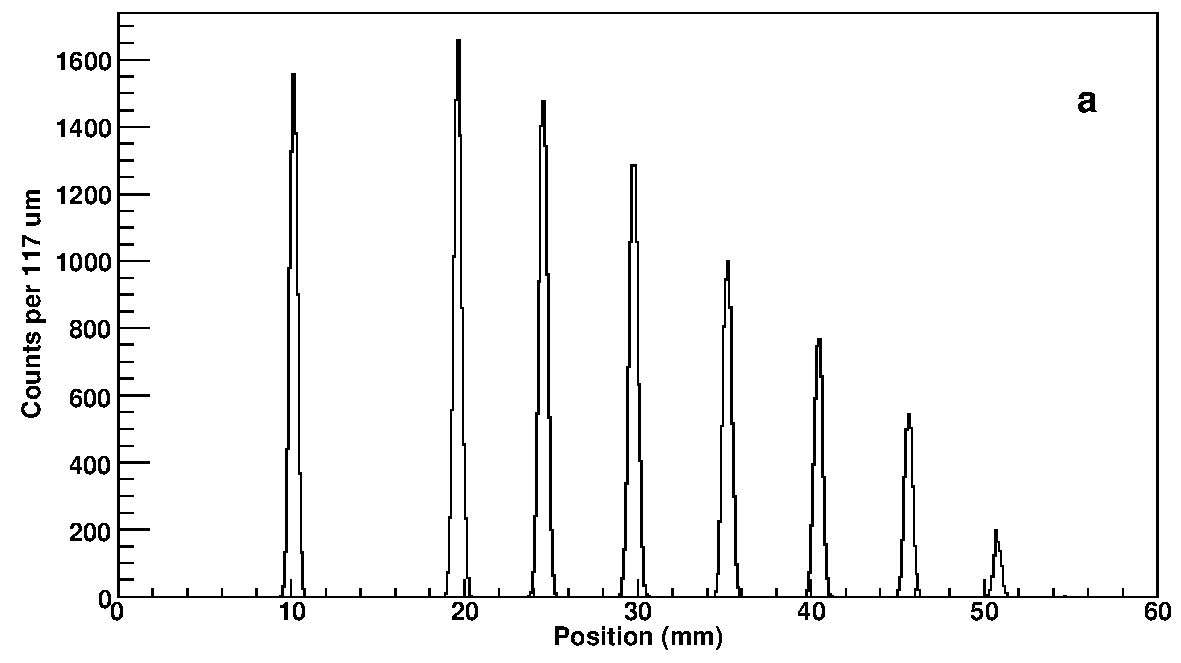
\includegraphics[height=0.45\textheight,width=\linewidth,keepaspectratio]{Figures/out3}
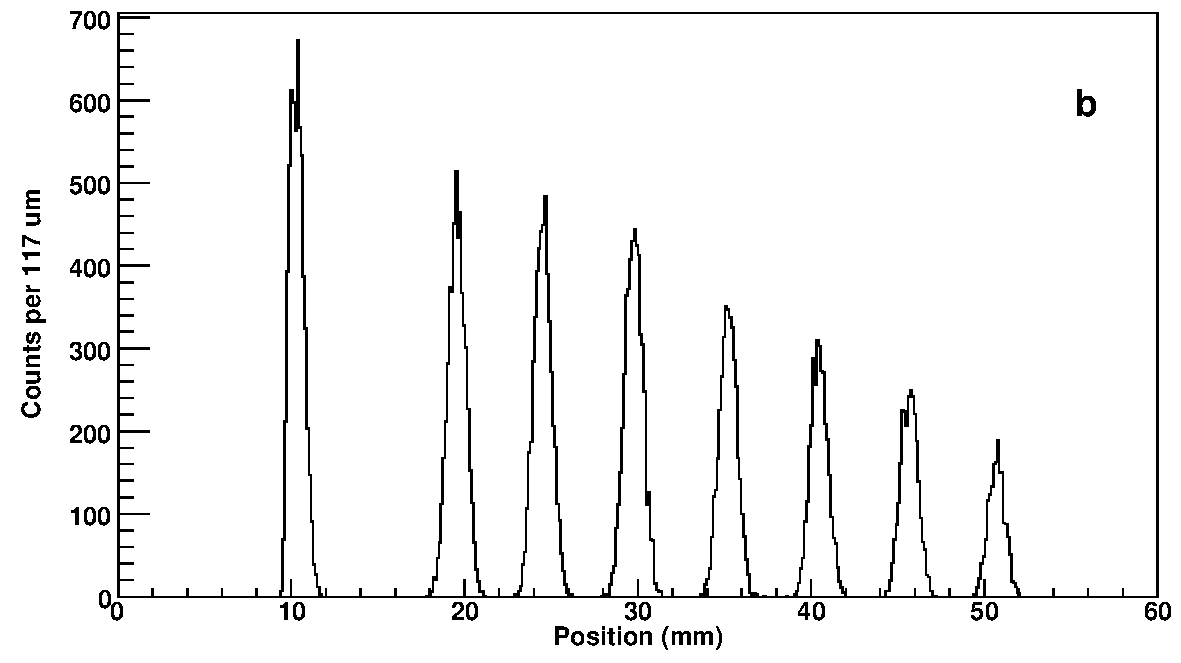
\includegraphics[height=0.45\textheight,width=\linewidth,keepaspectratio]{Figures/out4}
\caption[Position resolution of protons from ($p$,$p$) at two energies in a HELIOS PSD]{Position resolution of protons from ($p$,$p$) at two energies in a HELIOS PSD. Protons are elastically scattered from $^{12}$C.  (a) For $E_1=5.0$\,MeV, the average position resolution is 0.532\,mm~FWHM.  (b) For $E_1=2.0$\,MeV, the position resolution is 1.17\,mm~FWHM.  This figure appears similar form in Ref.~\cite{Lighthall_2010}.}
\label{psd_pos}
\end{figure}

\begin{figure}%
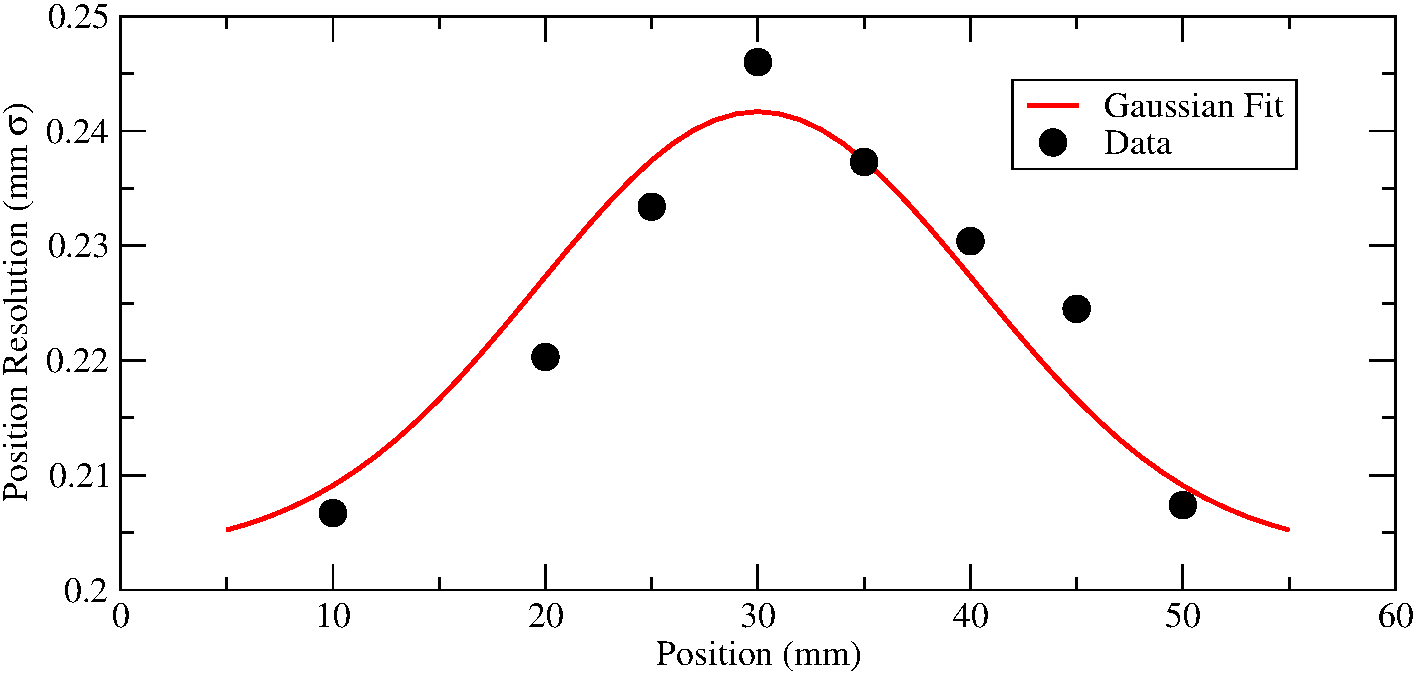
\includegraphics[width=\columnwidth]{resolution}%
\caption[Detector resolution as a function of position for scattered protons at 5\,MeV]{Detector resolution as a function of position for scattered protons at 5\,MeV.  Peak widths measured from the spectrum shown in Fig.~\ref{psd_pos}(a).  The position resolution varies $\pm6$\% over the length of the detector.}%
\label{res_fig}%
\end{figure}

\begin{figure}
\centering
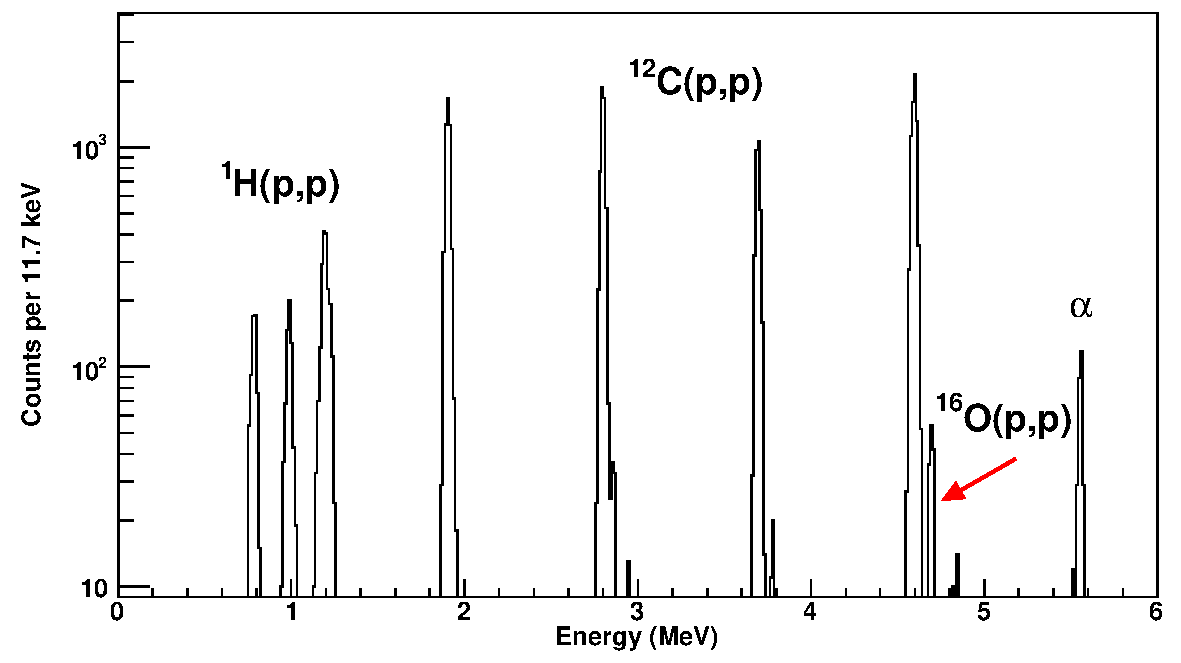
\includegraphics[height=0.5\textheight,width=\linewidth,keepaspectratio]{Figures/out5}
\caption[Energy resolution spectrum of a HELIOS PSD for the slit located at 30\,mm]{Energy resolution spectrum of a HELIOS PSD for the slit located at 30\,mm.  This position corresponds to a proton scattering angle of $60^\circ$ in the laboratory frame.  The peaks near 1\,MeV correspond to the protons from $^1$H(p,p) with an energy resolution of 52.8\,keV~FWHM.  The peaks in the range of 2-5\,MeV 
 correspond to protons from $^{12}$C(p,p) with an energy resolution of 35.5\,keV~FWHM.  The peak near 4.7\,MeV 
 (indicated with an arrow) corresponds to protons from $^{16}$O(p,p).  The peak near 5.5\,MeV correspond to $\alpha$ 
 particles from a $^{241}$Am calibration source with an energy resolution of 27.1\,keV~FWHM.  This figure appears similar form in Ref.~\cite{Lighthall_2010}.
 }
\label{psd_energy}
\end{figure}

\subsubsection{Time}
Additional measurements using ($p$,$p$) scattering were made in March 2007 to evaluate the timing response of the detectors.  One of the HELIOS silicon detectors was installed at a scattering angle of $\theta_\mathrm{lab}=45^\circ$ relative to the beam line. A scintillator with a photomultiplier tube was also installed 45$^\circ$ relative to the beam axis, such that the opening angle between the detectors was 90$^\circ$.  The experimental setup is shown in Fig.~\ref{scat_setup}.  
A polyvinyl formal (Formvar$\textsuperscript{\textregistered}$) foil was used for its hydrogen content for ($p$,$p$) scattering.  With the detector arranged in such a way, coincident elastic scattering events may be detected.  A time to amplitude converter (TAC) was used to measure the difference in time-of-flight between protons detected in the scintillator and those in the silicon detector.  Fig.~\ref{time_tests} is a composite of the energy measured in the silicon detector at four different proton beam energies plotted as a function of the TAC signal.

\begin{figure*}%
\centering
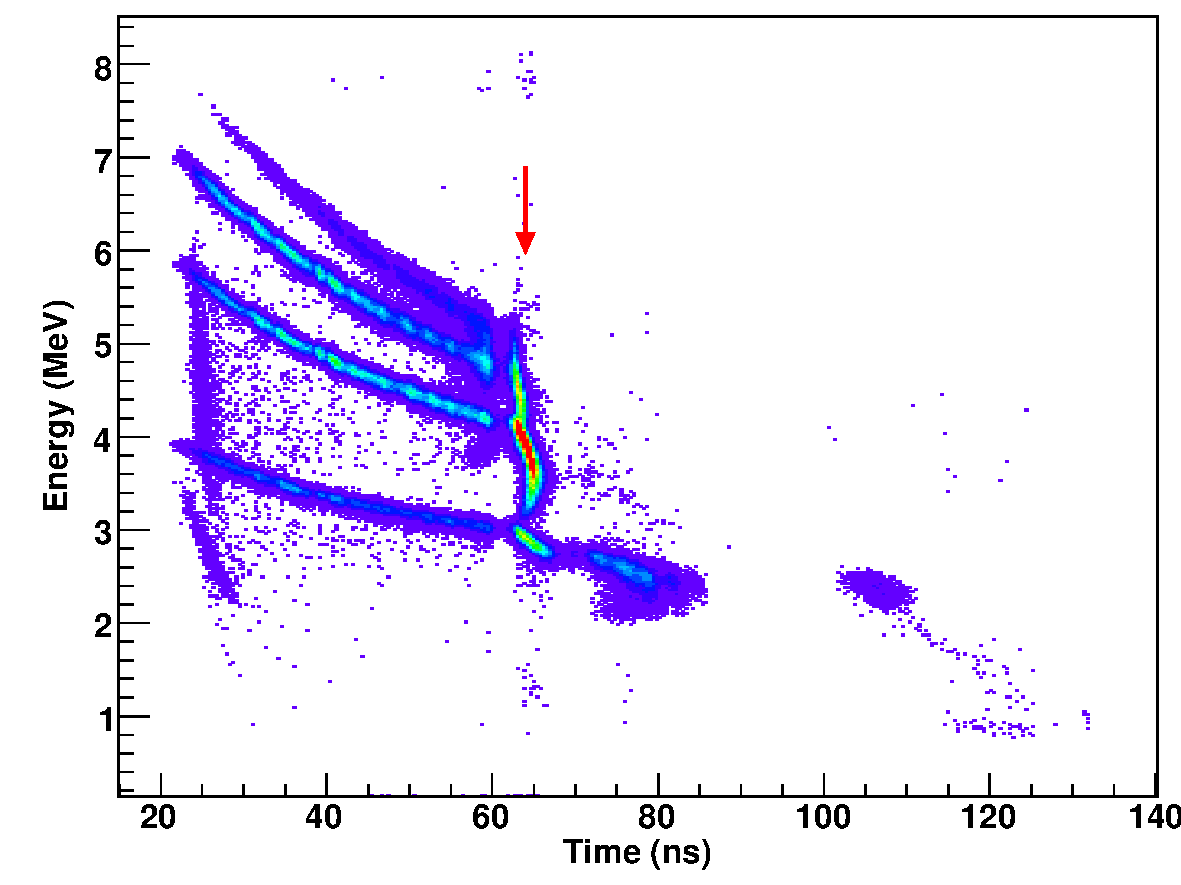
\includegraphics[width=\columnwidth]{timetest}%
\caption[Characteristic timing spectrum for a HELIOS PSD]{Characteristic timing spectrum for a HELIOS PSD. Energy versus TAC signal for protons from ($p$,$p$) scattering at four different beam energies $E_1=5$, 7.5, 9, 10\,MeV.  The width of the timing locus near 64\,ns (arrow) corresponding to coincidence events broadens from 1\,ns~FWHM to over 3\,ns~FWHM with decreasing energy.}%
\label{time_tests}%
\end{figure*}

As discussed in Ref.~\cite{Bennett_1992}, the timing response of a position-sensitive detector varies with both energy and position.  The slower rise times of the energy signal both at lower energies and towards the center of the detector lead to a broadening of the timing signal.  This effect is present in the data shown in Fig.~\ref{time_tests}.  The timing locus near 64\,ns (indicated by the arrow) broadens with decreasing energy. Near 5.0\,MeV the detectors have a time resolution of approximately 1.11\,ns~FWHM.  The width of the timing signal increases steadily to 3.28\,ns~FWHM near 2.5\,MeV.  The timing resolution required for particle identification is only on the order of 10\,ns, which these detectors easily meet.  The position dependence of the timing response was not assessed in this series of measurements, however, this feature is discussed in Chapt.~\ref{calib} which covers the calibration of the detectors.

\subsubsection{Length}
\label{sss:leng}
A longer PSD was also characterized to assess the possibility of reducing the number of detectors making up the array.  Tests were conducted with a Design X2 PSD manufactured by Micron Semiconductor which had an active area $22.2 \times 94.8$\,mm$^2$.
%\note{I'm not sure if this is the actual detector we used, but it matches its characteristics.}
  As with the previous characterization measurements, protons were elastically scattered from a $^{12}$C foil at a variety of beam energies.  The detector was located at a radius 125\,mm  away from the beam axis such that protons scattered at $\theta_\mathrm{lab}=60^\circ$ were normally incident on the detector. A mask covered the detector which had 0.5\,mm wide slits spaced every 5.0\,mm.  Fig.~\ref{big_psd_test} shows the results of these tests.  Whereas the 50.5\,mm-long detector has a position resolution of $0.532 \pm 0.031$\,mm~FWHM at $E_1=5$\,MeV, the 94.8\,mm-long detector has a position resolution of $1.370 \pm 0.065$\,mm~FWHM.  Furthermore, at energies below about 1.6\,MeV the position resolution of the longer detector degrades below 5\,mm---which is consistent with the manufacturer's stated resolution of 5650\,$\mu$m---making it unsuitable for many HELIOS applications.  However, the 50.5\,mm detectors \textit{are} suitable for HELIOS, meeting the necessary design requirements.
\begin{figure*}%
\centering
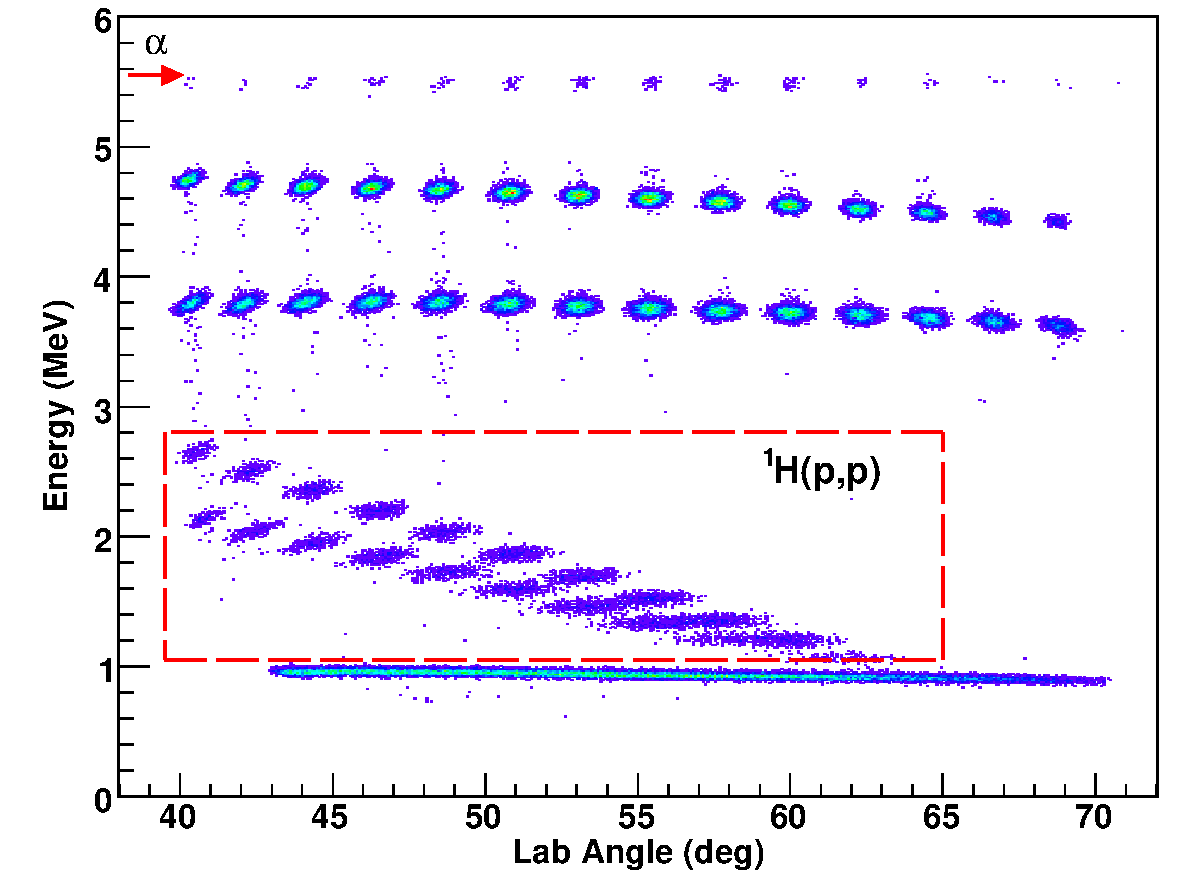
\includegraphics[width=\linewidth]{bigout1}
\caption[Characteristic energy versus scattering angle plot for a 94.8\,mm-long detector]{Characteristic energy versus scattering angle plot for a 94.8\,mm-long detector.  Protons were elastically scattered from a $^{12}$C foil at three different beam energies $E_1=1$, 4, 5\,MeV.  The detector was covered by a mask with 0.50\,mm wide slits every 5\,mm.  Elastic scattering from $^1$H (box) is present due to water in the target (faint loci corresponding to $^{16}$O($p$,$p$) can also be seen).  The series of points at 5.5\,MeV (arrow) correspond to $\alpha$ particles from a $^{241}$Am calibration source.  At low energy, the position resolution is less than the slit separation; thus the structure due to the slits is not present in the locus near 1\,MeV.}
\label{big_psd_test}
\end{figure*}
\section{The Array}
\label{array}
The detector array discussed in this section is a working prototype which was developed to demonstrate the feasibility of the HELIOS concept.  Two ostensibly opposing design requirements had to be reconciled in the design of the HELIOS detector array.  The first is that the silicon detector array must have a small outer radius such that particles are detected as close as possible to the solenoid axis.  A small radius of detection $\rho_0$ reduces the effects discussed in \S\,\ref{finite}, such as the degree by which particle flight times are reduced from the cyclotron period.  The minimum diameter of the detector array would be on the order of the width of the detector, in this case 12\,mm.

The second design requirement of the detector array is a large inner diameter.  This feature is necessary to permit transmission of the beam through the array to the target.  The inner opening of the array must also be large enough to allow for small misalignments in the beam which are encountered during the process of tuning the accelerator.  With this consideration in mind, the inner diameter of the detector array should be on the order of a typical tuning collimator; about 10\,mm.  Combining both of these design features suggests a thin-walled structure with a regular-polygonal cross section.

\subsection{Construction}
Extruded aluminum profiles are well-suited to this application because they are light-weight, rigid, and can be made in a variety of lengths and cross sections.  The core of the HELIOS silicon detector array uses a portion of an extruded aluminum 80/20 brand T-slotted profile.  The T-slotted profiles consist of a hollow core, square in cross section, and four T-slot flanges for mounting hardware (see Fig.~\ref{80/20}).  In the original design of the silicon detector array, the T-slot flanges were to be utilized as the mounting point for the detector array.  These flanges were ultimately removed along the entire length of the extrusion.

\begin{figure*}
\begin{center}
\fbox{
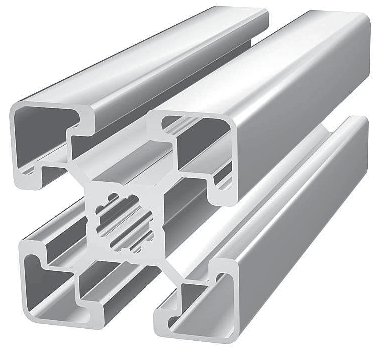
\includegraphics[width=0.5\textwidth,height=.375\textwidth,keepaspectratio]{Figures/45-4545-Lite}}
\hspace{\stretch{1}}
\fbox{

\includegraphics[width=0.5\textwidth,height=.375\textwidth,keepaspectratio]{Figures/DSC00541_bw}}
\end{center}
\caption[The 80/20 T-slotted profile used in the construction of the HELIOS array]{The 80/20 T-slotted profile used in the construction of the HELIOS array.  (Left) Cross section view of the 80/20-brand 45\,mm square extruded aluminum T-slotted profile 45-4545-Lite which is used as the central support of the detector array. (Right) The author machining the profile to expose the square core for use in the detector array.  Photo by N.~J.\ Goodman, \photodate\formatdate{16}{2}{2007}.}
\label{80/20}
\end{figure*}

Using the central core of a T-slotted profile as the mounting surface of the silicon detector array required that the T-slot flanges to be removed.  The T-slotted profile was machined down on a lathe to a diameter of 20.32\,mm, as shown in Fig.~\ref{80/20} (right).  The resulting structure is a 680\,mm long, 15.96\,mm square aluminum rod with a 10\,mm diameter central bore which forms the central support of the HELIOS detector array.
It was intended from the onset of the array's design that it would eventually be replaced.  Therefore, some of the components of the prototype array were designed to be compatible with an updated array.  In this instance, 
the overall length of the array was designed to ultimately accommodate 10 5\,mm-long detectors for the proposed updated array.  

The prototype array has six detectors on each side of the array.  The detectors are installed on the central support of the array in a modular fashion with each side of the array constituting an individual module.  The detectors reside on four printed circuit (PC) boards, each with dimensions of 388\,mm $\times$ 18\,mm.  Each detector is affixed to an electrical contact on the PC board with conductive epoxy.  The PC boards are assembled with the detectors aligned end-to-end, separated by bonding pads, with \label{typo4}% six detectors on each PC board and 
an average gap between wafers of 3.0\,mm\footnote{The value reported in Ref.~\cite{Lighthall_2010} (2.4\,mm) is off by a factor of 4/5, based on a schematic that unintentionally omitted one of the gaps.}.  Table~\ref{det_pos} shows the precise positions of each detector.  During the construction of the array, a precision mounting jig was used to aid in the placement of the detectors on the PC boards and to align them to better than 200\,$\mu$m~\cite{Marley_2008}.  Each position contact on the detectors are electrically connected to the contacts on the PC board by two aluminum bonding wires.  The three signals from the detectors are carried along traces in the PC board to where they are read out from one end of the board using two 34-pin connectors.  Each of these connectors attaches to a ribbon cable.


\begin{table}%
\centering
\begin{tabular}{cd{2}d{1}d{2}d{1}d{2}d{1}}
\hline \multirow{2}{*}{Det.}&
\multicolumn{2}{c}{Near}&&
\multicolumn{2}{c}{Far}&
\\ \cline{2-3}\cline{5-6}
&\multicolumn{1}{c}{Wafer}&
\multicolumn{1}{c}{Sensor}&
\multicolumn{1}{c}{Center}&
\multicolumn{1}{c}{Sensor}&
\multicolumn{1}{c}{Wafer}&
\multicolumn{1}{c}{Gap}\\ \hline \hline
%6&25.25&0&-2.75&50.5&53.25&\multicolumn{1}{c}{---}\\
%5&84.25&59&56.25&109.5&112.25&3.0\\
%4&143.25&118&115.25&168.5&171.25&3.0\\
%3&202.15&176.9&174.15&227.4&230.15&2.9\\
%2&261.45&236.2&233.45&286.7&289.45&3.3\\
%1&320.05&294.8&292.05&345.3&348.05&2.6\\
6&-2.75&0.0&25.25&50.5&53.25&\multicolumn{1}{c}{---}\\
5&56.25&59.0&84.25&109.5&112.25&3.0\\
4&115.25&118.0&143.25&168.5&171.25&3.0\\
3&174.15&176.9&202.15&227.4&230.15&2.9\\
2&233.45&236.2&261.45&286.7&289.45&3.3\\
1&292.05&294.8&320.05&345.3&348.05&2.6\\


\hline
\end{tabular}
\caption[Positions of the silicon detectors as mounted on the silicon detector array]{Positions of the silicon detectors as mounted on the silicon detector array.  Position are given in mm relative to the active area of the target-end of  Detector 6.  These values are based on the engineering schematic of the PC board and have been measured to be accurate to within 200\,$\mu$m.}
\label{det_pos}
\end{table}

\begin{figure*}[t]
\centering
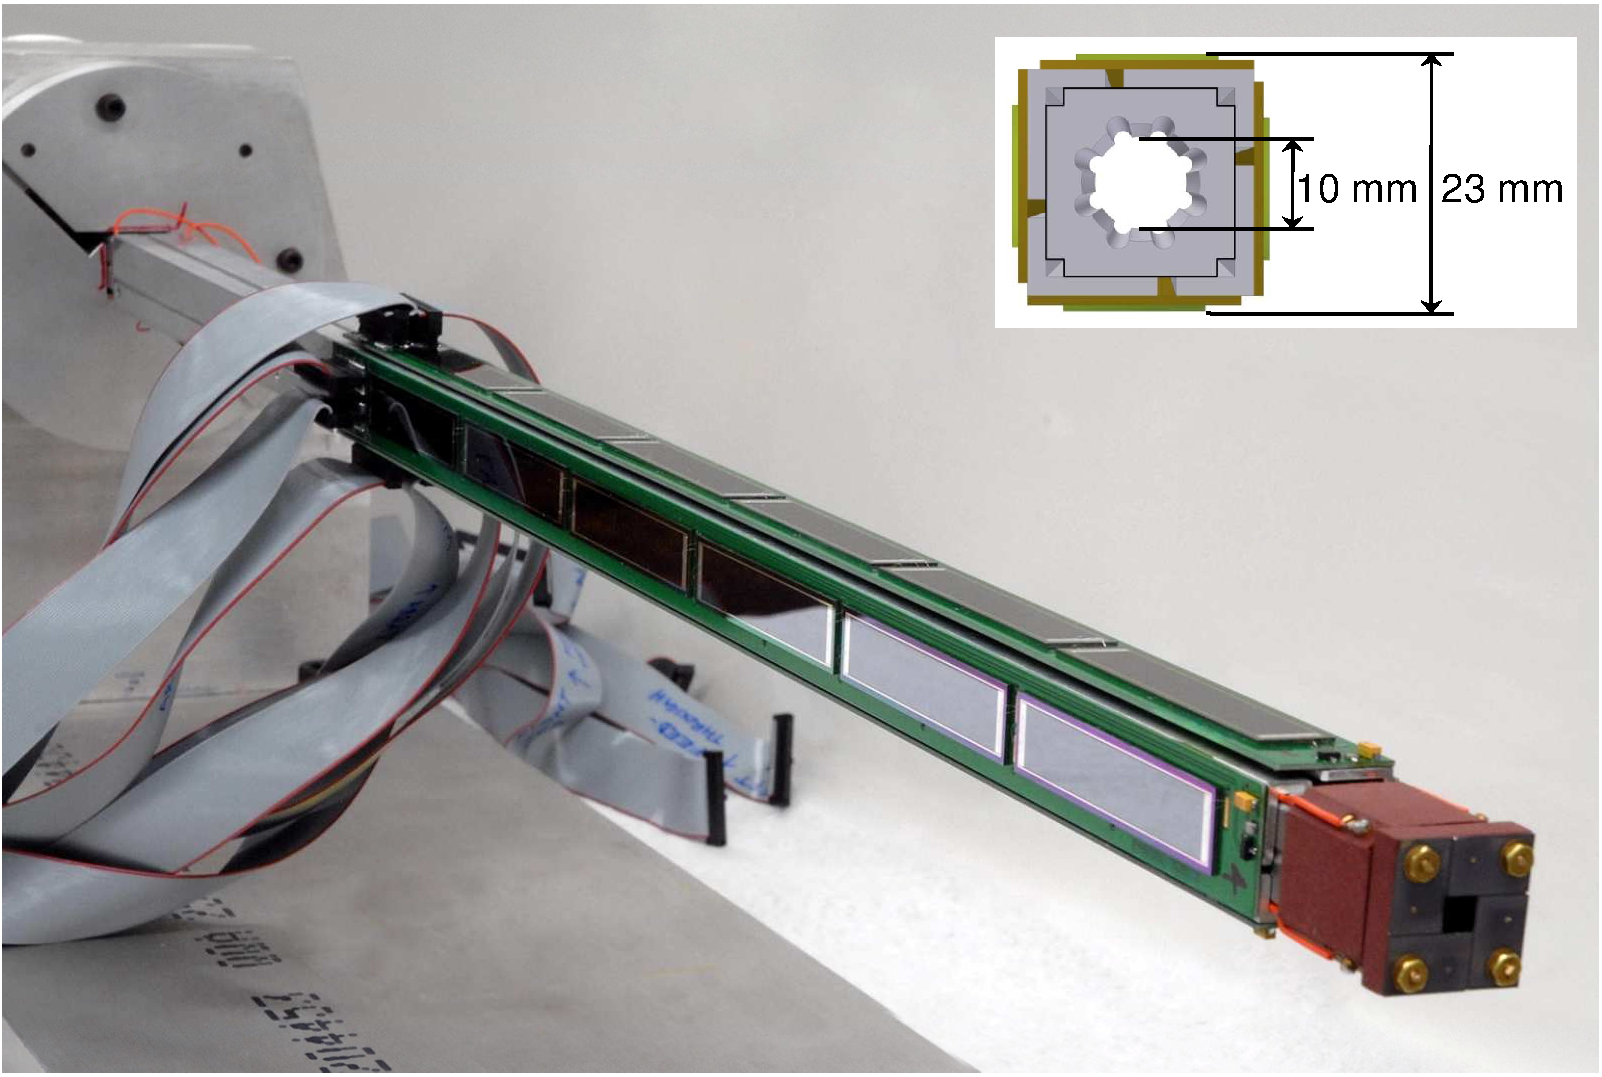
\includegraphics[width=\linewidth]{../NIM_Paper/Figures/DSC_0592ecs_inset3}
\caption[The HELIOS silicon detector array after full assembly mounted in its transport stand]{The HELIOS silicon detector array after full assembly mounted in its transport stand.  The 5\,mm $\times$ 5\,mm four-element collimator can be seen at the target-end of the array. At the far end of the array the eight 34-conductor ribbon cables which carry the detector signals are bundled together.  Photo by A.~H.\ Wuosmaa, \photodate\formatdate{17}{10}{2008}.  The inset shows a schematic drawing of the array cross section.  This figure also appears in Ref.~\cite{Lighthall_2010}.}
\label{array_pic}
\end{figure*}

Each of the modular PC boards described above is epoxied to aluminum L-brackets 573\,mm long.  The L-brackets are mounted to each side of the array support and are held in place with several screws.  The target-end of the array support is capped with an attachment for a removable 4-jaw slit which is used in beam tuning.  The signals from the slits run along the array in the space provided by the rounded edges of the array support (see Fig.~\ref{array_pic}).  On the far end of the array, about 100\,mm of the central support is exposed as a clamping surface to hold the array in place.  The fully assembled HELIOS detector array is shown in Fig.~\ref{array_pic}.  The array has a square cross section 23\,mm on a side and is 710\,mm long with the active length covering 345\,mm. 

  The aluminum end of the array is held inside a liquid-cooled copper block, shown in Fig.~\ref{block}.  The mechanical contact between the array and the cooling block is made with thermoelectric coolers (``Peltier coolers''), which can supply additional cooling.  The electrical connections for the Peltier coolers and the cooling lines both occupy their own 4.45\,cm feedthrough.  Neither system was utilized during the commissioning experiment.  However, circulating a chilled ethyl glycol solution allows the array to be cooled to temperatures below 0$^\circ$\,C.  The temperature of the array is monitored by four small temperature sensors, one at the target-end of each PC board making up the detector array (see Fig.~\ref{pcb}).  Further cooling from the Peltier coolers is possible, but as of this writing, the system needs to be redesigned to utilize the additional cooling.  

\begin{figure}%
\centering
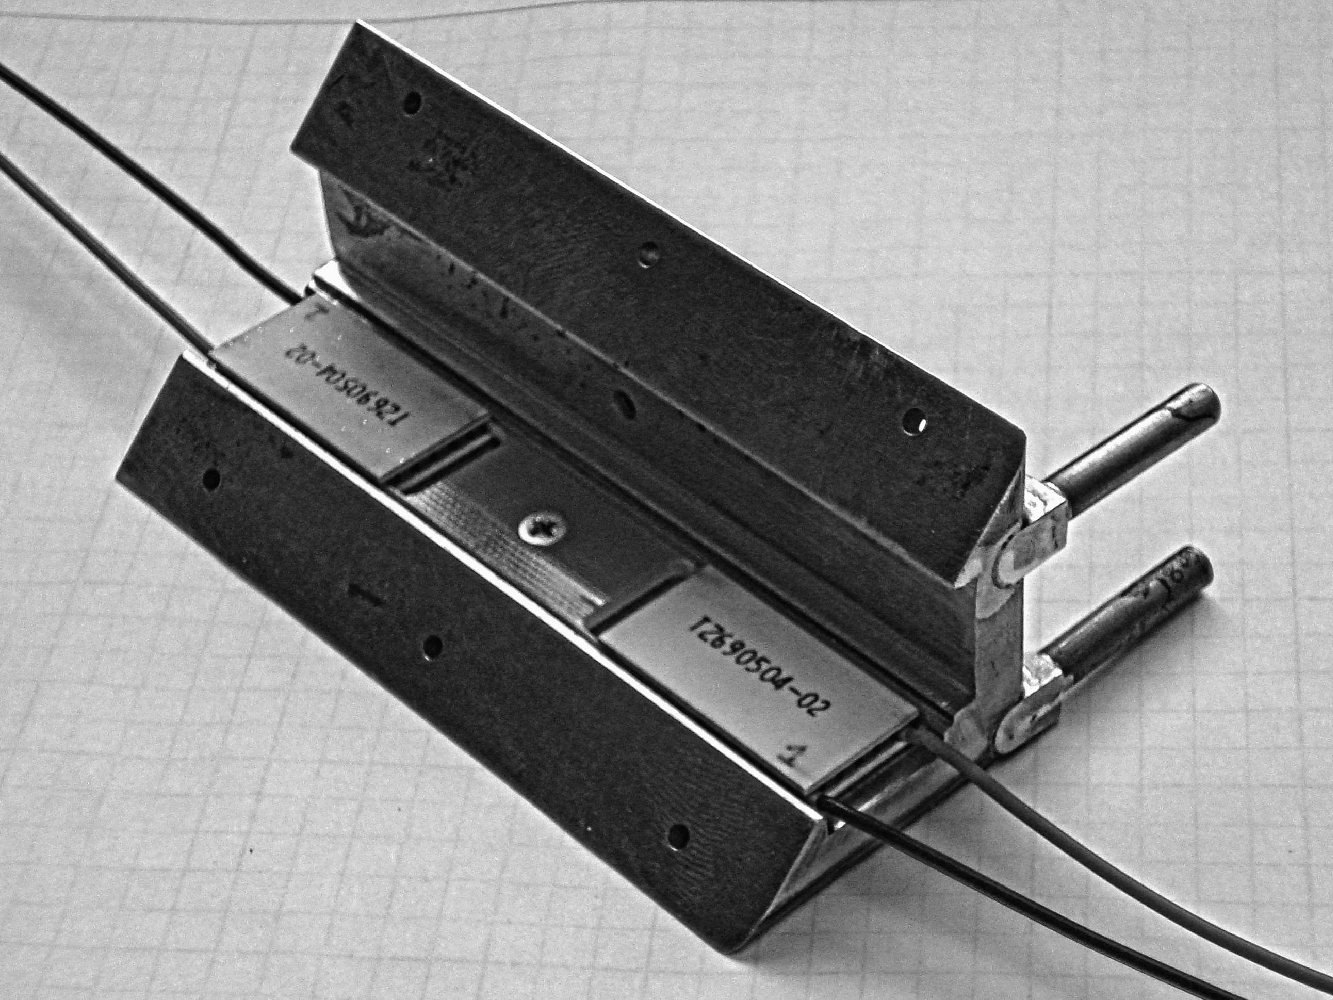
\includegraphics[width=\columnwidth, height=0.4\textheight, keepaspectratio]{DSC01400}%
\caption[One half of the copper cooling block which clamps the silicon array]{One half of the copper cooling block which clamps the silicon array.  As shown, two of the four Peltier coolers are installed, held in place by a fiberglass bracket.  The inlet and outlet of the liquid cooling channel are shown at right.}%
\label{block}%
\end{figure}

\subsection{Alignment}
The cooling block is seated inside an insulating fiberglass frame which is fitted to the end of a support tube (see Fig.~\ref{align}).  The support tube is part of a linear bearing which allows the detector array to be translated axially within the solenoid volume over a range of about 400\,mm.  The recent installation of a chain drive on the linear bearing allows this adjustment to be made while the system is under vacuum.

\begin{figure}%
\centering
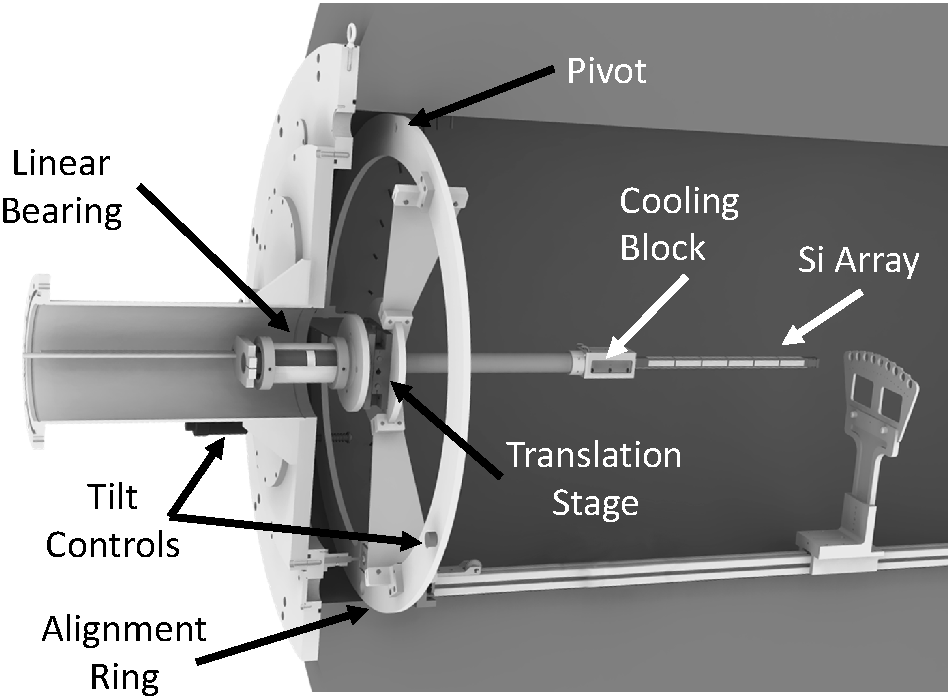
\includegraphics[width=0.75\linewidth,height=0.4\textheight,keepaspectratio]{alignment2}%
\caption{Enlargement of Fig.~\ref{schematic} detailing the alignment structures.}%
\label{align}%
\end{figure}

In order for the transmission of the beam through the array, the array must be aligned with respect to the beam axis to better than 2.5\,mm, or 2\,mrad, along its length.  The collimator at the target-end of the array is used to align front of the array while a removable centering jig is installed at the end of the support tube furthest away from the detector array.  These two reference points are aligned to the beam line optically using a surveying telescope.  The linear bearing system---and thus the array---are mounted to the alignment ring via a translation stage which provides motion perpendicular to the solenoid axis.  The entire alignment ring is suspended by a pivot at the top of the solenoid chamber, occupying one of the 4.45\,cm feedthroughs.  Two mechanical feedthroughs occupy the positions 120$^\circ$ from vertical (at 4 o'clock and 8 o'clock) allowing the alignment ring to be tilted about the pivot in order to align the array angularly.  Iterating these two alignment motions allows the array to be optically aligned to the beam axis with a precision of $<1$\,mm.  With the addition of the array chain drive, the array alignment hardware use 4 of the 12 4.45\,cm feedthroughs on the end of the solenoid holding the array.

%\subsubsection{Discussion}
